\Chapter{Relations I}
\Lettrine{One} of mathematicians' most essential abilities is noticing and describing relationships. We come across many patterns and links that could be characterised by relations in our everyday lives, like a relation between a parent and child or between an employer and an employee. The idea of relationships between sets is essential, and we will look at their properties here.

\section{What is a Relation?}
A high-level explanation of a relation is simply a way to `create a connection' between items in two sets. However, the abstract definition of a relation is much less enlightening.

\begin{definition}[Relation]
    Let $X$ and $Y$ be sets. A \term{relation from $X$ to $Y$}\index{relation} is a subset of $X \times Y$.

    Let $R$ be a relation, $x \in X$, and $y \in Y$. We say that \term{$x$ is related to $y$ by $R$}\index{related to} (or that \term{$x$ is $R$-related to $y$}), denoted $x\mathrel{R}y$, if and only if $(x, y) \in R$. We write $x\not\mathrel{R}y$ if and only if $(x, y) \notin R$.

    If there is no confusion of what relation we are talking about, we can just say that \term{$x$ is related to $y$}.
\end{definition}
\begin{remark}[$n$-ary Relations]
    Strictly speaking, what we have defined above is a \term{binary relation}\index{relation!binary}, since it only involves the Cartesian product of two sets. A more general type of relation that could be studied is a \term{$n$-ary relation}\index{relation!$n$-ary}, which is a subset of a Cartesian product of $n$ sets. In particular, for sets $A_1$, $A_2$, \dots, $A_n$, an $n$-ary relation on those sets is a subset of $A_1 \times A_2 \times \cdots \times A_n$. However, we will solely be working with binary relations in this book, and thus the term ``relation'' shall only be used to describe binary relations.
\end{remark}

This is clearly way too abstract of a definition to see how this captures the idea of `creating connections' between set elements, so let's take a look at some concrete examples.

\begin{example}[The ``lived in'' Relation]\label{example:lived-in-relation}
    Let $M$, a subset of the set of all mathematicians, be
    \[
        \{\text{Peano}, \text{Cantor}, \text{Dedekind}, \text{Russell}, \text{Euler}, \text{Hilbert}\}
    \]
    and let $C$, a subset of the set of all countries, be
    \[
        \{\text{Italy}, \text{Switzerland}, \text{Russia}, \text{Germany}, \text{France}\}.
    \]
    Then we can define $R$ to be the ``lived in'' relation. In particular,
    \begin{align*}
        R &= \{(\text{Peano}, \text{Italy}), (\text{Cantor}, \text{Russia}), (\text{Cantor}, \text{Germany}),\\
        &\quad\quad(\text{Dedekind}, \text{Germany}), (\text{Euler}, \text{Switzerland}),\\
        &\quad\quad(\text{Euler}, \text{Germany}), (\text{Euler}, \text{Russia}), (\text{Hilbert}, \text{Germany})\}.
    \end{align*}

    We can show this relation diagrammatically.
    \begin{figure}[H]
        \centering
        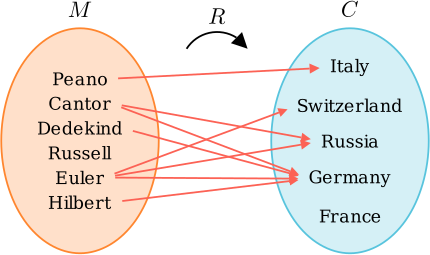
\includegraphics[height=3.75cm]{images/part-1/relations-1/lived-in.png}
        \caption{Arrow Diagram of $R$}
    \end{figure}

    On the left is the set $M$, and on the right is the set $C$. The arrows shows how they are related. For example, the arrow from ``Peano'' points to ``Italy'' since Giuseppe Peano lived in Italy. Notice that Bertrand Russell did not live in any of the countries in $C$, and that no mathematician in $M$ lived in France.
\end{example}

\begin{example}[The ``is less than'' Relation]\label{example:is-less-than-relation}
    Let $A = \{0, 1, 2\}$ and $B = \{1, 2, 3\}$. Define the relation $R$ such that
    \[
        x\mathrel{R}y \iff x < y
    \]
    for all $x \in A$ and $y \in B$. Then $0\mathrel{R}1$, $0\mathrel{R}2$, $0\mathrel{R}3$, $1\mathrel{R}2$, $1\mathrel{R}3$, and $2\mathrel{R}3$. However we see $1 \not\mathrel{R} 1$, $2 \not\mathrel{R} 1$, and $2 \not\mathrel{R} 2$. Thus
    \[
        R = \{(0, 1), (0, 2), (0, 3), (1, 2), (1, 3), (2, 3)\}.
    \]

    Again, we may show this relation diagrammatically.
    \begin{figure}[H]
        \centering
        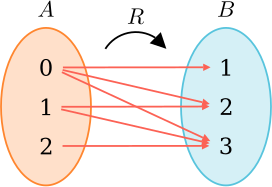
\includegraphics[height=2.75cm]{images/part-1/relations-1/less-than.png}
        \caption{Arrow Diagram of $R$}
    \end{figure}
\end{example}

Relations may also be performed on the same set.

\begin{definition}[Relation on a Set]
    A \term{relation $R$ on a set $A$}\index{relation!on a set} is a relation from $A$ to $A$. That is, $R$ is a subset of $A^2$.
\end{definition}
\begin{remark}[$n$-ary Relation on a Set]
    Likewise, a $n$-ary relation on a set $A$ is a subset of $A^n$.
\end{remark}

\begin{example}[Relation on a Set]
    Let $A = \{3, 4, 5, 6, 7\}$ and define a relation $R$ on $A$ such that
    \[
        x\mathrel{R}y \iff x - y \text{ is an even number}
    \]
    for all $x, y \in A$. Then one sees that
    \begin{align*}
        R &= \{(3, 3), (3, 5), (3, 7), (4, 4), (4, 6), (5, 3), (5, 5),\\
        &\quad\quad(5, 7), (6, 4), (6, 6), (7, 3), (7, 5), (7, 7)\}.
    \end{align*}

    We can, of course, show this relationship using the standard arrow diagram, but we can also use a directed graph (a graph with directed edges) to represent it.

    \begin{figure}[H]
        \begin{subfigure}{0.45\textwidth}
            \centering
            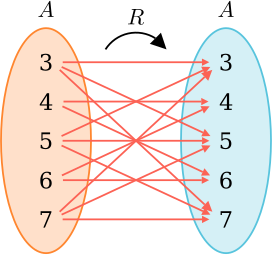
\includegraphics[width=3.5cm]{images/part-1/relations-1/relation-on-a-set_arrow-diagram.png}
            \caption{Arrow Diagram}
        \end{subfigure}
        \hfill
        \begin{subfigure}{0.45\textwidth}
            \centering
            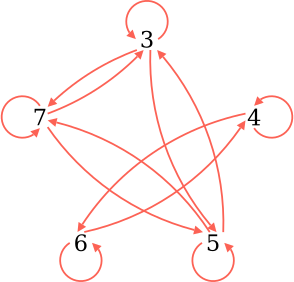
\includegraphics[width=3.5cm]{images/part-1/relations-1/relation-on-a-set_directed-graph.png}
            \caption{Directed Graph}
        \end{subfigure}
        \caption{Diagrammatic Representations of $R$} 
    \end{figure}
\end{example}

\begin{exercise}[Relation Discriminator]
    Let $A = \{2, 3, 4, 5\}$ and $B = \{2, 4, 6, 8\}$. Which of the following sets are relations from $A$ to $B$? Which of the following sets are relations on $A$?
    \begin{partquestions}{\alph*}[2]
        \item $R_1 = \emptyset$
        \item $R_2 = \{(2, 2), (3, 3), (4, 4)\}$
        \item $R_3 = \{(2, 2), (3, 4), (4, 8), \linebreak(5, 6), (5, 8)\}$
        \item $R_4 = \{2, 3, 4\}$
        \item $R_5 = \{(2, 4), (4, 6), (6, 8)\}$
        \item $R_6 = A^2$
        \item $R_7 = B^2$
    \end{partquestions}
\end{exercise}

We end this section by looking at the equality of relations.

\begin{definition}[Equality of Relations]\label{definition:equality-of-relations}
    Let $A$, $B$, $C$, and $D$ be sets. Let $R$ be a relation from $A$ to $B$ and $S$ a relation from $C$ to $D$. The two relations $R$ and $S$ are equal\index{relation!equal} if and only if $A = C$, $B = D$, and the set $R$ equals the set $S$.
\end{definition}
\begin{remark}[A Relation as an Ordered Triple]
    In light of the above definition of relation equality, we could define a relation from the set $A$ to the set $B$ to be an ordered triple $(A, B, R)$, where $R \subseteq A \times B$. We stick to our definition of a relation as a subset of $A \times B$ instead.
\end{remark}

\section{Properties of Relations}
Let us now look at some properties of relations.

\begin{definition}[Domain, Codomain, and Range]
    Let $X$ and $Y$ be sets and $R$ be a relation from $X$ to $Y$.
    \begin{itemize}
        \item The \term{domain}\index{domain}\index{relation!domain} of $R$ is the set $\{x \in X \vert \exists y \in Y \text{ s.t. } x \mathrel{R} y\}$.
        \item The \term{codomain}\index{codomain}\index{relation!codomain} of $R$ is the set $Y$.
        \item The \term{range}\index{range}\index{relation!range} of $R$ is the set $\{y \in Y \vert \exists x \in X \text{ s.t. } x \mathrel{R} y\}$.
    \end{itemize}
\end{definition}

\begin{example}
    Let $A = \{1,2,3\}$ and $B = \{2,4,9\}$. Let the relation $R$ be a relation from $A$ to $B$ such that
    \[
        x \mathrel{R} y \iff x^2 = y.
    \]
    In particular, we see that
    \[
        R = \{(2, 4), (3, 9)\}.
    \]
    The domain of $R$ is
    \begin{align*}
        &\{a \in A \vert \exists b \in B \text{ s.t. } a \mathrel{R} b\}\\
        &= \{a \in A \vert \exists b \in B \text{ s.t. } a^2 = b\}\\
        &= \{2, 3\}.
    \end{align*}

    The codomain of $R$ is the set $B$, which is $\{2,4,9\}$.

    The range of $R$ is
    \begin{align*}
        &\{b \in B \vert \exists a \in A \text{ s.t. } a \mathrel{R} b\}\\
        &= \{b \in B \vert \exists a \in A \text{ s.t. } a^2 = b\}\\
        &= \{4, 9\}.
    \end{align*}
\end{example}

Let us now look at the inverse of a relation.

\begin{definition}[Inverse of a Relation]
    Let $X$ and $Y$ be sets and $R$ be a relation from $X$ to $Y$. The inverse\index{relation!inverse} of $R$, denoted $R^{-1}$, is the relation from $Y$ to $X$ where $y \mathrel{R^{-1}} x$ if and only if $x \mathrel{R} y$ for any $x \in X$ and $y \in Y$. In other words,
    \[
        R^{-1} = \{(y, x) \in Y \times X \vert (x, y) \in X \times Y\}.
    \]
\end{definition}

\begin{example}[The ``is less than'' Relation and its Inverse]
    In \myref{example:is-less-than-relation}, we looked at the relation $R$ from the set $A = \{0, 1, 2\}$ to $B = \{1, 2, 3\}$ such that $x \mathrel{R} y \iff x < y$ for all $x \in A$ and $y \in B$. In particular, we found that
    \[
        R = \{(0, 1), (0, 2), (0, 3), (1, 2), (1, 3), (2, 3)\}.
    \]
    Therefore
    \begin{align*}
        R^{-1} &= \{(1, 0), (2, 0), (3, 0), (2, 1), (3, 1), (3, 2)\} & (\text{Swap } x \text{ and } y)\\
        &= \{(1, 0), (2, 0), (2, 1), (3, 0), (3, 1), (3, 2)\}. & (\text{Reordering})
    \end{align*}

    As usual, we may show these relations diagrammatically.
    \begin{figure}[H]
        \begin{subfigure}{0.45\textwidth}
            \centering
            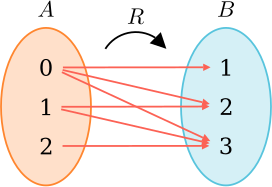
\includegraphics[width=3.5cm]{images/part-1/relations-1/less-than.png}
        \end{subfigure}
        \hfill
        \begin{subfigure}{0.45\textwidth}
            \centering
            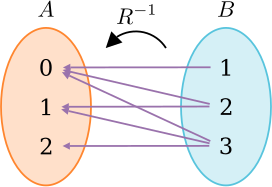
\includegraphics[width=3.5cm]{images/part-1/relations-1/less-than_inverse.png}
        \end{subfigure}
        \caption{Arrow Diagrams of $R$ and $R^{-1}$} 
    \end{figure}
    One sees that the arrow diagram for $R^{-1}$ is formed by reversing the arrows on the arrow diagram of $R$.
\end{example}

\begin{exercise}[Properties of the ``Divides'' Relation]
    \setlength{\parindent}{0pt}
    (\textit{Assume multiplication of integers is defined.})

    Let $S = \{2, 3, 4, 5, 6, 7, 8\}$. Define a relation $D$ on $S$ such that
    \[
        x \mathrel{D} y \iff \exists m \in S \text{ s.t. } y = mx
    \]
    for all $x, y \in S$.

    \begin{partquestions}{\roman*}
        \item List the elements in $D$. Hence list the elements in $D^{-1}$.
        \item List the elements in the
        \begin{partquestions}{\alph*}
            \item domain of $D$;
            \item codomain of $D$; and
            \item range of $D$.
        \end{partquestions}
    \end{partquestions}
\end{exercise}

\begin{exercise}[Inverse Relation of Inverse Relation]
    Let $A$ and $B$ be sets. Let $R$ be a relation from $A$ to $B$. Prove that
    \[
        \left(R^{-1}\right)^{-1} = R.
    \]
\end{exercise}

\section{Composition of Relations}
We may sometimes want to find the overall relationship between two sets after a sequence of relations. This motivates the concept of composing relations.

\begin{definition}[Composition of Relations]
    Let $A$, $B$, and $C$ be sets. Let $R$ and $S$ be relations from $A$ to $B$ and $B$ to $C$ respectively. The \term{composition of $R$ with $S$}\index{relation!composition}, written $S \circ R$, is a relation from $A$ to $C$ where
    \[
        a (\mathrel{S \circ R}) c \iff \exists b \in B \text{ s.t. } ((a \mathrel{R} b) \land (b \mathrel{S} c))
    \]
    for all $a \in A$ and $c \in C$. In other words,
    \[
        S \circ R = \{(a, c) \in A \times C \vert \exists b \in B \text{ s.t. } ((a, b) \in R \land (b, c) \in S)\}.
    \]
\end{definition}
% \begin{remark}[Order Matters]
%     $S \circ R$ and $R \circ S$ are different. The former means that we apply $R$ \textbf{before} $S$, while the latter means that we apply $S$ \textbf{before} $R$. The reason we write ``$S \circ R$'' to mean that $R$ comes before $S$ is to match the notation for function composition (which will be covered later).
% \end{remark}

\begin{example}[The ``lived in continent'' Relation]\label{example:lived-in-content-relation}
    In \myref{example:lived-in-relation}, we defined the sets
    \begin{align*}
        M &= \{\text{Peano}, \text{Cantor}, \text{Dedekind}, \text{Russell}, \text{Euler}, \text{Hilbert}\},\\
        C &=\{\text{Italy}, \text{Switzerland}, \text{Russia}, \text{Germany}, \text{France}\}, \text{ and}\\
        R &= \{(\text{Peano}, \text{Italy}), (\text{Cantor}, \text{Russia}), (\text{Cantor}, \text{Germany}),\\
        &\quad\quad(\text{Dedekind}, \text{Germany}), (\text{Euler}, \text{Switzerland}),\\
        &\quad\quad(\text{Euler}, \text{Germany}), (\text{Euler}, \text{Russia}), (\text{Hilbert}, \text{Germany})\},
    \end{align*}
    where $R$ is, in particular, a relation from $M$ to $C$ called the ``lived in'' relation. Now let the set $A$, a subset of all continents (``areas''), be
    \[
        \{\text{Europe}, \text{North America}, \text{Asia}\}.
    \]
    Define the relation $S$ from $C$ to $A$ to be the ``country of'' relation where
    \begin{align*}
        S &= \{(\text{Italy}, \text{Europe}), (\text{Switzerland}, \text{Europe}), (\text{Russia}, \text{Asia}),\\
        &\quad\quad(\text{Germany}, \text{Europe}), (\text{France}, \text{Europe})\}.
    \end{align*}
    Thus the composition of $R$ with $S$ (i.e., $S \circ R$) is the ``lived in continent'' relation. In particular,
    \begin{align*}
        S \circ R &= \{(\text{Peano}, \text{Europe}), (\text{Cantor}, \text{Europe}), (\text{Cantor}, \text{Asia})\\
        &\quad\quad (\text{Dedekind}, \text{Europe}), (\text{Euler}, \text{Europe}), (\text{Euler}, \text{Asia})\\
        &\quad\quad (\text{Hilbert}, \text{Europe})\}.
    \end{align*}

    Like in \myref{example:lived-in-relation}, we can show this relation diagrammatically.
    \begin{figure}[H]
        \centering
        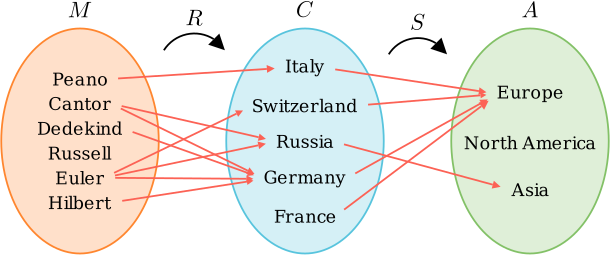
\includegraphics[height=3.5cm]{images/part-1/relations-1/lived-in-continent_separate.png}
        \caption{Arrow Diagram of $R$ and $S$}
    \end{figure}
    Removing the intermediate set $C$ yields the following arrow diagram.
    \begin{figure}[H]
        \centering
        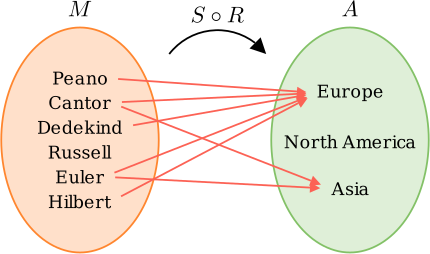
\includegraphics[height=3.5cm]{images/part-1/relations-1/lived-in-continent_composed.png}
        \caption{Arrow Diagram of $S \circ R$}
    \end{figure}
\end{example}

\pagebreak  % TODO: Can we remove this ugly (in terms of the code) page break?

\begin{example}[Composition of a Relation on a Set]
    Let $A = \{0, 1, 2, 3, 4\}$. Define the relation $R$ on $A$ such that $x\mathrel{R}y \iff x < y$ for all $x, y \in A$. Thus
    \begin{align*}
        R &= \{(0, 1), (0, 2), (0, 3), (0, 4), (1, 2),\\
        &\quad\quad(1, 3), (1, 4), (2, 3), (2, 4), (3, 4)\}.
    \end{align*}
    Subsequently, one sees that
    \[
        R\circ R = \{(0, 2), (0, 3), (0, 4), (1, 3), (1, 4), (2, 4)\}.
    \]
    
    We can draw the directed graphs of both relations.
    \begin{figure}[H]
        \begin{subfigure}{0.45\textwidth}
            \centering
            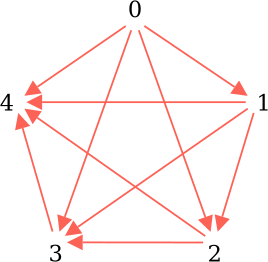
\includegraphics[width=3.5cm]{images/part-1/relations-1/composition-of-relation-on-a-set_original.png}
            \caption{Directed Graph of $R$}
        \end{subfigure}
        \hfill
        \begin{subfigure}{0.45\textwidth}
            \centering
            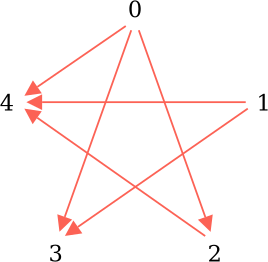
\includegraphics[width=3.5cm]{images/part-1/relations-1/composition-of-relation-on-a-set_composed.png}
            \caption{Directed Graph of $R \circ R$}
        \end{subfigure}
        \caption{Directed Graphs of $R$ and $R \circ R$} 
    \end{figure}
\end{example}
% \begin{remark}[$n$ Repeated Compositions of a Relation on a Set]
%     In the above example, the relation $R \circ R$ can be more concisely written as $R^2$. Likewise, the relation $R \circ (R \circ R)$ can be written as $R^3$, and so on.
% \end{remark}

\begin{exercise}[Properties of Compositions]
    Let $A$, $B$, and $C$ be 3 distinct non-empty sets. Let $R$ and $S$ be relations from $A$ to $B$ and $B$ to $C$ respectively such that $R$ and $S$ are both non-empty. Which of the following statements is/are always true?
    \begin{partquestions}{\alph*}
        \item The domain of $S \circ R$ can be empty.
        \item The domain of $S \circ R$ is $A$.
        \item The domain of $S \circ R$ can be $A$.
        \item The codomain of $S \circ R$ can be empty.
        \item The codomain of $S \circ R$ is $C$.
        \item The codomain of $S \circ R$ can be $B$.
        \item The range of $S \circ R$ can be empty.
        \item The range of $S \circ R$ is $C$.
        \item The range of $S \circ R$ can be $C$.
    \end{partquestions}
\end{exercise}

Let us now consider the inverse of a composed relation.

\begin{example}[The ``lived in continent'' Relation's Inverse]
    Recall in \myref{example:lived-in-content-relation} we have the sets
    \begin{align*}
        M &= \{\text{Peano}, \text{Cantor}, \text{Dedekind}, \text{Russell}, \text{Euler}, \text{Hilbert}\},\\
        C &=\{\text{Italy}, \text{Switzerland}, \text{Russia}, \text{Germany}, \text{France}\}, \text{ and}\\
        A &= \{\text{Europe}, \text{North America}, \text{Asia}\}
    \end{align*}
    and the relations
    \begin{align*}
        R &= \{(\text{Peano}, \text{Italy}), (\text{Cantor}, \text{Russia}), (\text{Cantor}, \text{Germany}),\\
        &\quad\quad(\text{Dedekind}, \text{Germany}), (\text{Euler}, \text{Switzerland}),\\
        &\quad\quad(\text{Euler}, \text{Germany}), (\text{Euler}, \text{Russia}), (\text{Hilbert}, \text{Germany})\}
    \end{align*}
    and
    \begin{align*}
        S &= \{(\text{Italy}, \text{Europe}), (\text{Switzerland}, \text{Europe}), (\text{Russia}, \text{Asia}),\\
        &\quad\quad(\text{Germany}, \text{Europe}), (\text{France}, \text{Europe})\}
    \end{align*}
    from $M$ to $C$ and $C$ to $A$ respectively. We found that their composition was
    \begin{align*}
        S \circ R &= \{(\text{Peano}, \text{Europe}), (\text{Cantor}, \text{Europe}), (\text{Cantor}, \text{Asia})\\
        &\quad\quad (\text{Dedekind}, \text{Europe}), (\text{Euler}, \text{Europe}), (\text{Euler}, \text{Asia})\\
        &\quad\quad (\text{Hilbert}, \text{Europe})\}.
    \end{align*}
    The inverse is thus
    \begin{align*}
        (S \circ R)^{-1} &= \{(\text{Europe}, \text{Peano}), (\text{Europe}, \text{Cantor}), (\text{Asia}, \text{Cantor})\\
        &\quad\quad (\text{Europe}, \text{Dedekind}), (\text{Europe}, \text{Euler}), (\text{Asia}, \text{Euler})\\
        &\quad\quad (\text{Europe}, \text{Hilbert})\}.
    \end{align*}

    \begin{figure}[H]
        \begin{subfigure}{0.4875\textwidth}
            \centering
            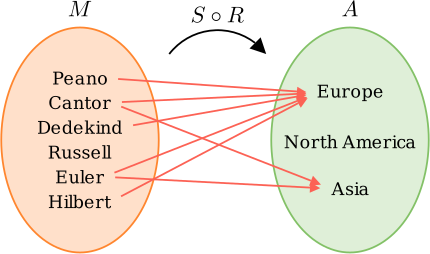
\includegraphics[width=5cm]{images/part-1/relations-1/lived-in-continent_composed.png}
        \end{subfigure}
        \hfill
        \begin{subfigure}{0.4875\textwidth}
            \centering
            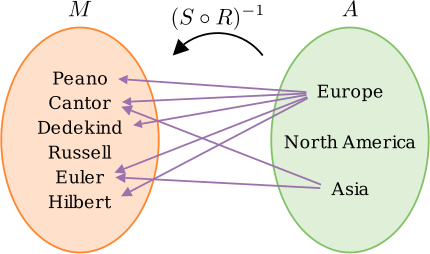
\includegraphics[width=5cm]{images/part-1/relations-1/lived-in-continent-inverse_composed.png}
        \end{subfigure}
        \caption{Arrow Diagrams of $S \circ R$ and $(S \circ R)^{-1}$} 
    \end{figure}

    Now consider the relations $R^{-1}$ and $S^{-1}$. Their arrow diagrams can be combined as one.
    \begin{figure}[H]
        \centering
        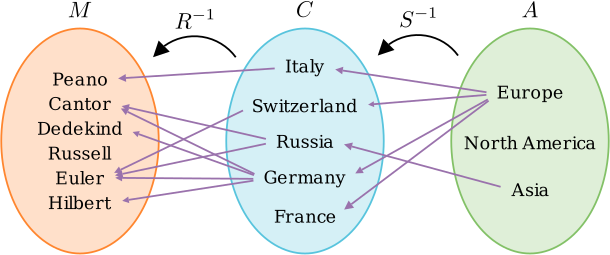
\includegraphics[height=3.5cm]{images/part-1/relations-1/lived-in-continent-inverse_separate.png}
        \caption{Arrow Diagram of $R^{-1}$ and $S^{-1}$}
    \end{figure}
    From this diagram, we can see another method for finding $(S\circ R)^{-1}$ -- by first using the inverse of $S$ and then the inverse of $R$. In other words, we see that $(S \circ R)^{-1} = R^{-1} \circ S^{-1}$.
\end{example}

\begin{wrapfigure}{r}{0.35\textwidth}
    \centering
    
\includegraphics[width=2.75cm]{images/part-1/relations-1/shoes-and-socks.jpg}
\end{wrapfigure}

This observation that $(S\circ R)^{-1} = R^{-1} \circ S^{-1}$ is a key property of the inverse of a composition of two relations, informally called the \term{shoes and socks theorem}. The intuition behind this property is similar to that of putting on socks and then shoes. To remove them both, you first have to take off your shoes (i.e., the second thing that you put on) and then take off your socks (i.e., the first thing that you put on). Likewise, to undo the effect of two relations $R$ and then $S$, we first have to undo $S$ and then undo $R$.

\begin{theorem}[Shoes and Socks (Relations)]\label{theorem:shoes-and-socks-relations}\index{shoes and socks}
    Let $A$, $B$, and $C$ be sets, and let $R$ and $S$ be relations from $A$ to $B$ and $B$ to $C$ respectively. Then
    \[
        (S \circ R)^{-1} = R^{-1} \circ S^{-1}.
    \]
\end{theorem}
\begin{proof}
    See \myref{exercise:shoes-and-socks-relations} (later).
\end{proof}

Another property that the composition enjoys is associativity.

\begin{theorem}[Associativity of Composition (Relations)]\index{relation!composition!associativity}
    Let $A$, $B$, $C$, and $D$ be sets. Let $R$, $S$, and $T$ be relations from $A$ to $B$, $B$ to $C$, and $C$ to $D$ respectively. Then
    \[
        (T \circ S) \circ R = T \circ (S \circ R).
    \]
\end{theorem}
\begin{proof}
    We first note that $(T \circ S) \circ R \subseteq A \times D$ and $T \circ (S \circ R) \subseteq A \times D$. Now suppose $a \in A$ and $d \in D$. We see
    \begin{align*}
        &(a, d) \in (T \circ S) \circ R\\
        \iff& a \mathrel{((T \circ S) \circ R)} d\\
        \iff& \exists b \in B \text{ s.t. } (a \mathrel{R} b \land b \mathrel{(T\circ S)} d)\\
        \iff& \exists b \in B \text{ s.t. } (a \mathrel{R} b \land (\exists c \in C \text{ s.t. } (b \mathrel{S} c \land c \mathrel{T} d)))\\
        \iff& \exists b \in B, c \in C \text{ s.t. } (a \mathrel{R} b \land b \mathrel{S} c \land c \mathrel{T} d)\\
        \iff& \exists c \in C \text{ s.t. } ((\exists b \in B \text{ s.t. } (a \mathrel{R} b \land b \mathrel{S} c)) \land c \mathrel{T} d)\\
        \iff& \exists c \in C \text{ s.t. } (a \mathrel{(S \circ R)} c \land c \mathrel{T} d)\\
        \iff& a \mathrel{(T \circ (S \circ R))} d\\
        \iff& (a, d) \in T \circ (S \circ R).
    \end{align*}
    So any element in $(T \circ S) \circ R$ is also in $T \circ (S \circ R)$ and vice versa, thereby meaning that $(T \circ S) \circ R = T \circ (S \circ R)$.
\end{proof}

Since there is no distinction between $(T \circ S) \circ R$ and $T \circ (S \circ R)$, we can write ``$T \circ S \circ R$'' without any ambiguity.

\begin{exercise}[Composition Commutivity?]
    Let $A$ and $B$ be sets. Let $R$ and $S$ be relations from $A$ to $B$ and $B$ to $A$ respectively. Which of the following is/are true?
    \begin{partquestions}{\alph*}
        \item It is always the case that $S \circ R = R \circ S$.
        \item It is never the case that $S \circ R = R \circ R$.
        \item It is possible for $S \circ R = R \circ S$.
    \end{partquestions}
\end{exercise}

\begin{exercise}[Shoes and Socks]\label{exercise:shoes-and-socks-relations}
    Prove \myref{theorem:shoes-and-socks-relations}.
\end{exercise}

\begin{exercise}[Composition of Relation and its Inverse]
    Let $A$ and $B$ be sets and let $R$ be a relation from $A$ to $B$. Determine whether the following statement is true or false.
    \[
        R^{-1} \circ R \subseteq \{(x, y) \in A^2 \vert x = y\}.
    \]
    If it is true, prove it. Otherwise, give a counterexample.
\end{exercise}
